\documentclass{standalone}
\usepackage{tikz}
\usetikzlibrary{angles,quotes}

\begin{document}

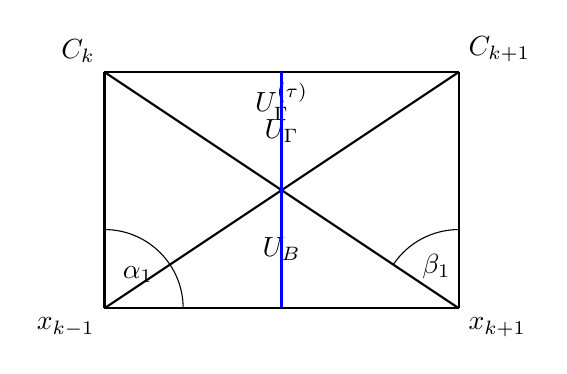
\begin{tikzpicture}[scale=1.5]
    % Define coordinates
    \coordinate (A) at (0,0);
    \coordinate (B) at (3,0);
    \coordinate (C) at (0,2);
    \coordinate (D) at (3,2);
    
    % Draw vertical lines
    \draw[thick] (A) -- (B);
    \draw[thick] (C) -- (D);
    
    % Draw horizontal lines
    \draw[thick] (A) -- (C);
    \draw[thick] (B) -- (D);
    
    % Draw diagonal lines
    \draw[thick] (A) -- (D);
    \draw[thick] (B) -- (C);
    
    % Draw angles
    \pic [draw, angle radius=1cm, "$\alpha_1$"] {angle = B--A--C};
    \pic [draw, angle radius=1cm, "$\beta_1$"] {angle = D--B--C};
    
    % Label points
    \node at (A) [below left] {$x_{k-1}$};
    \node at (B) [below right] {$x_{k+1}$};
    \node at (C) [above left] {$C_k$};
    \node at (D) [above right] {$C_{k+1}$};
    
    % Label U_B
    \node at (1.5, 0.5) {$U_B$};
    
    % Label U_Gamma
    \node at (1.5, 1.5) {$U_\Gamma$};
    \node at (1.5, 1.75) {$U_\Gamma^{(\tau)}$};
    
    % Draw blue line
    \draw[blue, thick] (1.5, 0) -- (1.5, 2);
\end{tikzpicture}

\end{document}